\documentclass{beamer}

\usepackage{graphicx}
\usepackage{numprint}

\mode<presentation>

\begin{document}

\begin{frame}
\frametitle{Ergon Data: All Customers}
\begin{itemize}
\item Billing data from approx. \numprint{472000} individual households
\item Most of households available after mid-2009 until early-2012
\end{itemize}
\begin{center}
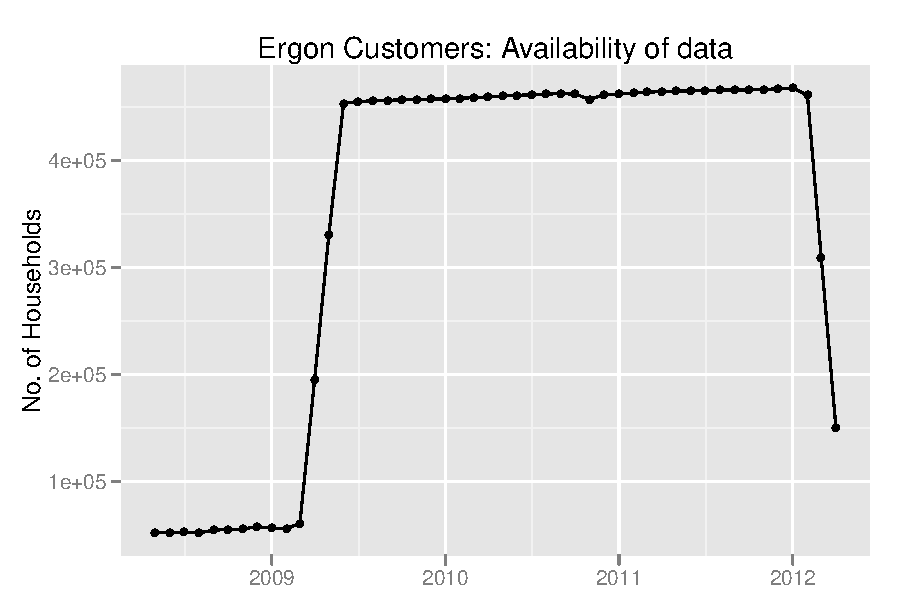
\includegraphics[width=0.8\textwidth]{figures/ErgonAvailDataFilled}
\end{center}
\end{frame}

\begin{frame}
\frametitle{Ergon Data: Program Participants}
\begin{itemize}
\item Approx. \numprint{57000} are program participants
\end{itemize}
\begin{center}
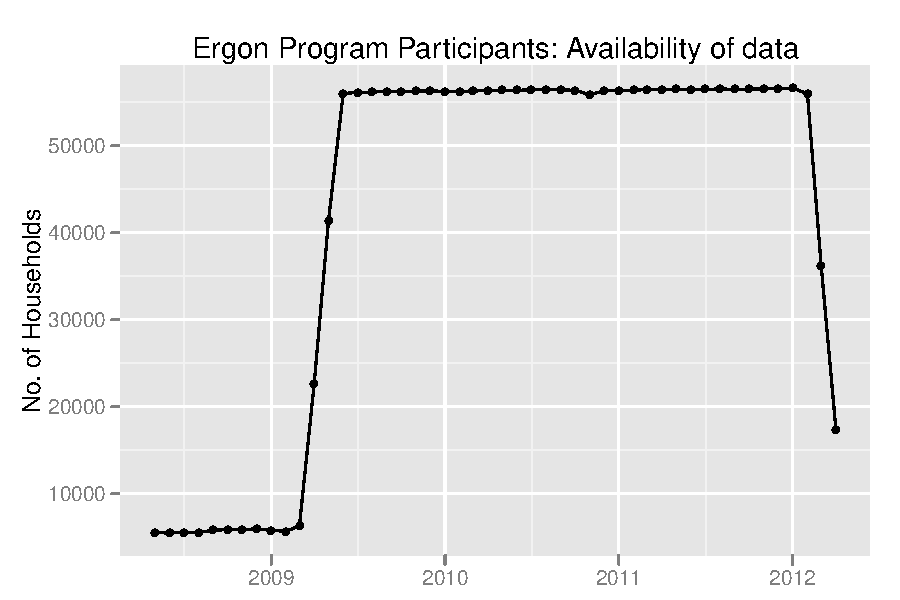
\includegraphics[width=0.8\textwidth]{figures/ErgonPartAvailData}
\end{center}
\end{frame}

\begin{frame}
\frametitle{Ergon Data: Participants By LGA}
\begin{center}
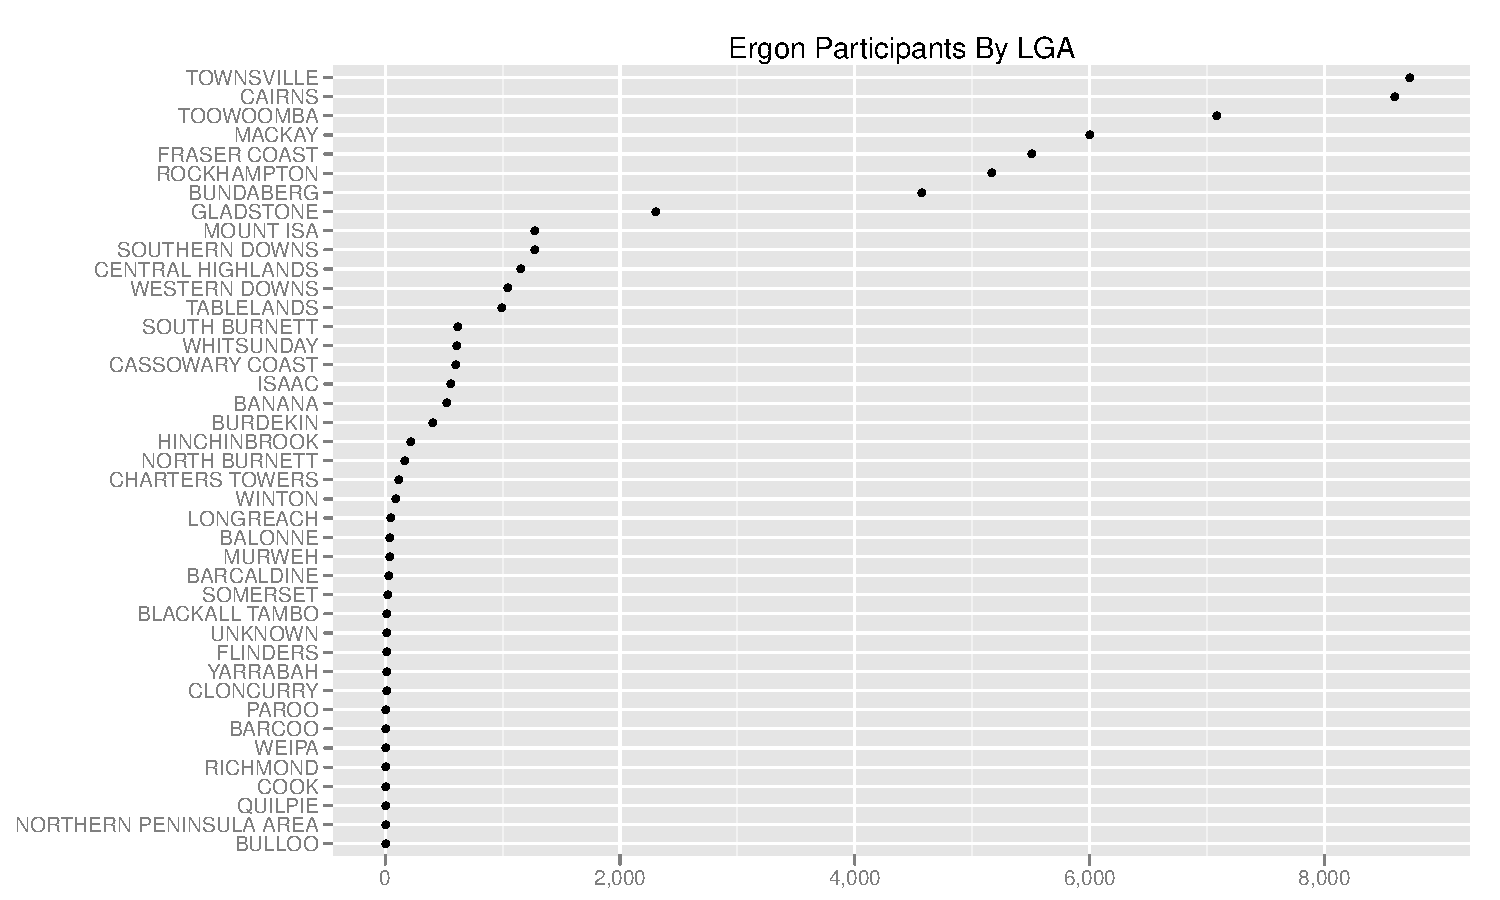
\includegraphics[width=1\textwidth]{figures/ErgonLGA}
\end{center}
\end{frame}

\begin{frame}
\frametitle{Energex Data: All Customers}
\begin{itemize}
\item Approx. \numprint{1234000} individual households
\item Data starting from April 2008 till October 2011
\end{itemize}
\begin{center}
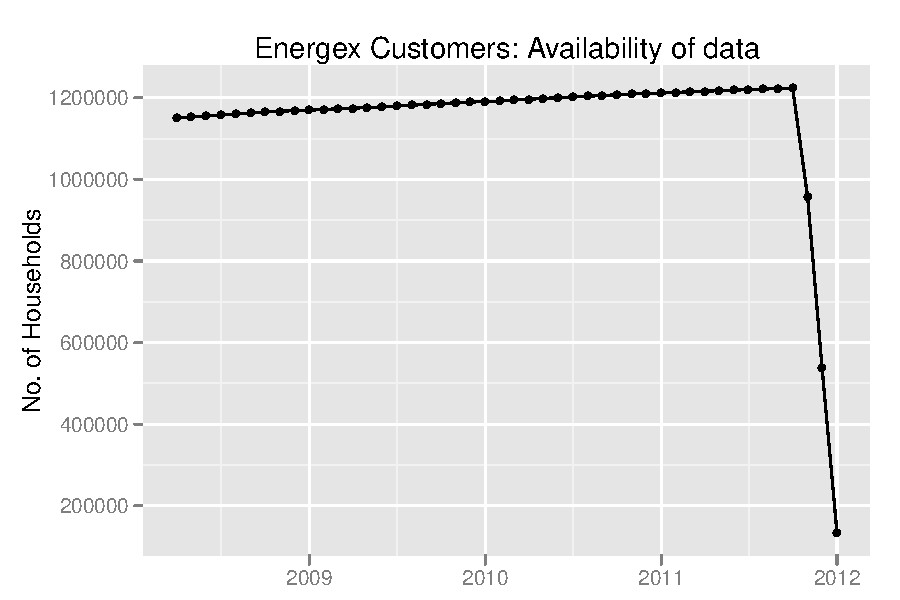
\includegraphics[width=0.8\textwidth]{figures/EnergexAvailData}
\end{center}
\end{frame}

\begin{frame}
\frametitle{Energex Data: Program Participants}
\begin{itemize}

\item Approx. \numprint{204000} participant households

\end{itemize}
\begin{center}
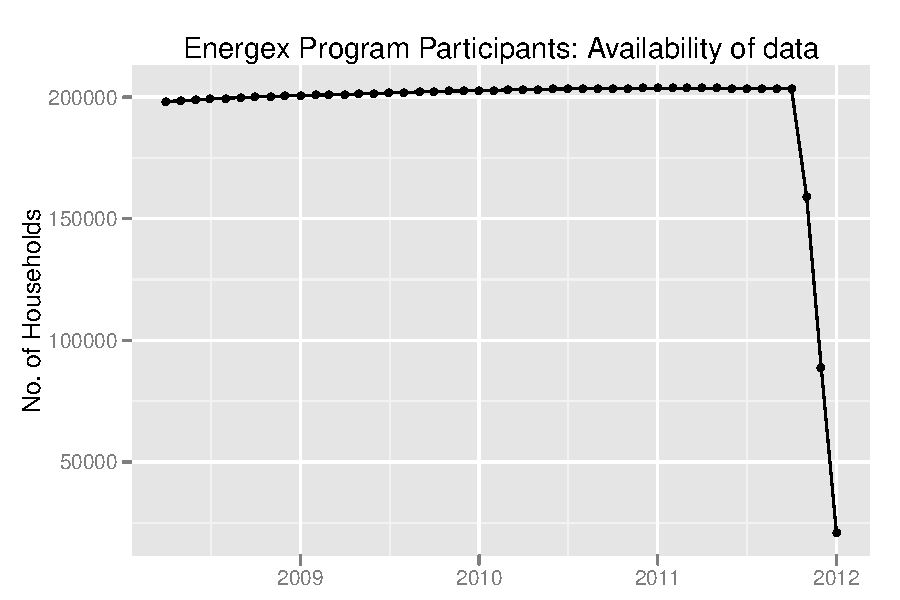
\includegraphics[width=0.8\textwidth]{figures/EnergexPartAvailData}
\end{center}
\end{frame}

\begin{frame}
\frametitle{Energex Data: Participants By LGA}
\begin{center}
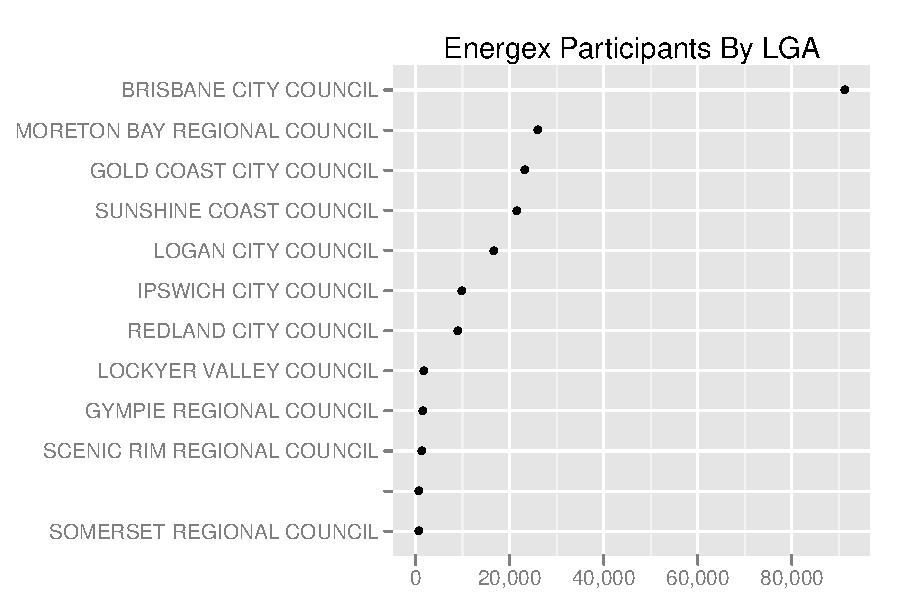
\includegraphics[width=1\textwidth]{figures/EnergexLGA}
\end{center}
\end{frame}

\begin{frame}
\frametitle{Average Consumption}
\begin{itemize}

\item From above we expect to see a difference in Ergon and Energex
participants/customers$\ldots$

\item But we also see a difference in participants and non-participants

\end{itemize}
\begin{center}
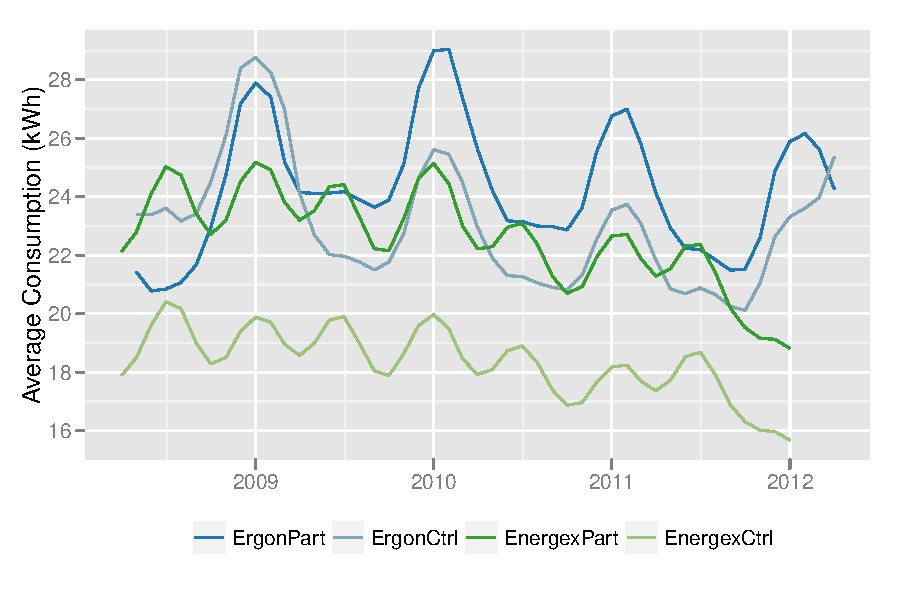
\includegraphics[width=0.9\textwidth]{figures/MeanConsumption}
\end{center}
\end{frame}

\begin{frame}
\frametitle{Average Consumption}
\begin{itemize}

\item A possible reason: property type of Energex participants
\begin{table}[h!]
\begin{center}
\begin{tabular}{lcccc}
\hline
& Unknown & Townhouse & Apart./Unit & House\\
\hline
Count & \numprint{1829} & \numprint{5835} & \numprint{11130} &
\numprint{185216}\\
\% & 0.90 &  2.86 & 5.46 & 90.79\\
\hline
\end{tabular}
\end{center}
\end{table}

\item The point: not safe to assume participants are a random sample of
non-participant households (COMMING BACK TO THIS)

\begin{center}
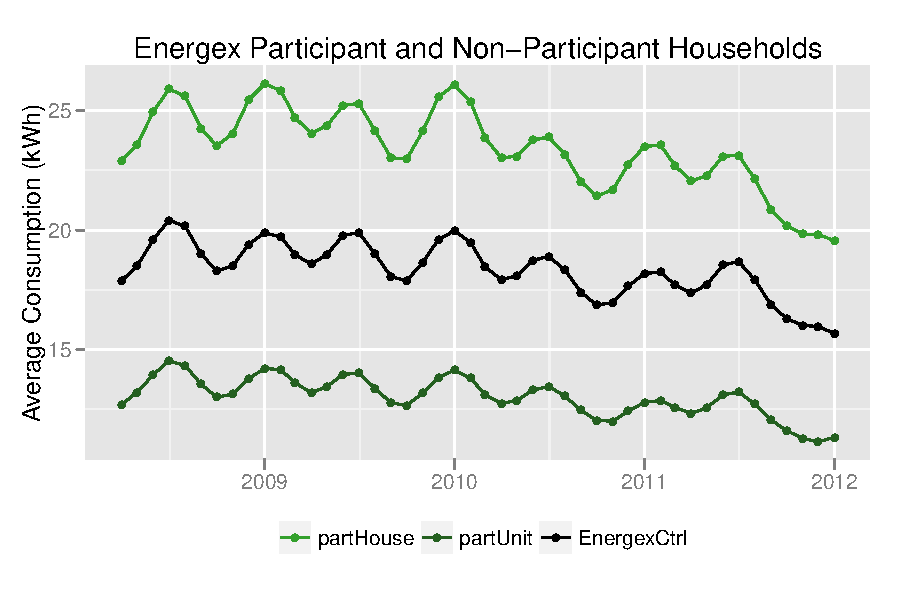
\includegraphics[width=0.7\textwidth]{figures/EnergexHouseUnits}
\end{center}
\end{itemize}
\end{frame}

\begin{frame}
\frametitle{Outliers 1}
\begin{itemize}
\item Example of two households consuming alot
\end{itemize}
\begin{center}
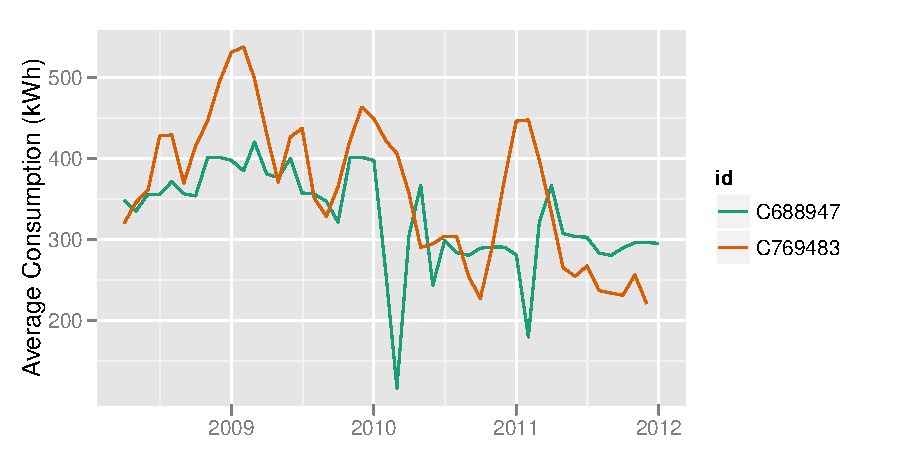
\includegraphics[width=1\textwidth]{figures/outlier1}
\end{center}
\end{frame}

\begin{frame}
\frametitle{Outliers 2}
\begin{itemize}
\item Example of two households with a spike
\end{itemize}
\begin{center}
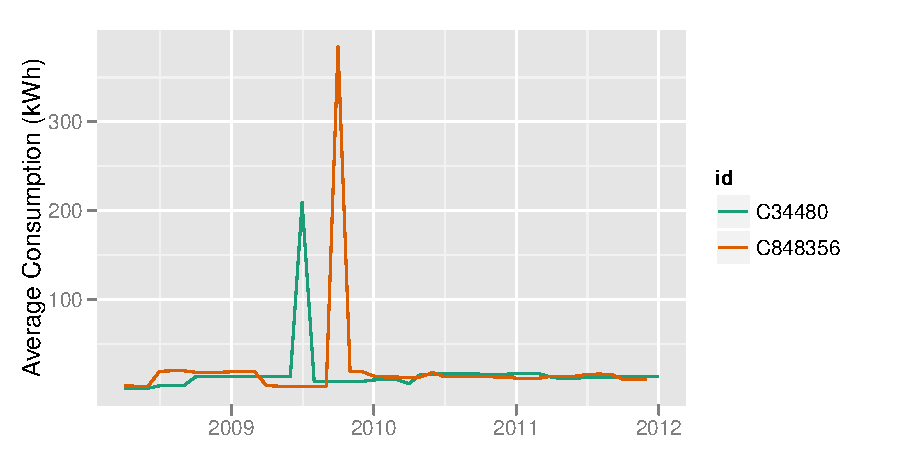
\includegraphics[width=1\textwidth]{figures/outlier2}
\end{center}
\end{frame}

\end{document}



